\documentclass[times,specification,annotation]{itmo-student-thesis}

\usepackage{icomma}

\usepackage{tikz}
\usepackage{systeme}
\usetikzlibrary{arrows}
\usepackage{filecontents}
\usepackage{fancybox}
\usepackage{array}
\usepackage{proof}
\usepackage{fontspec}


%% box для правил вывода
\newenvironment{calculus}
{\begin{center}\begin{Sbox}\begin{minipage}[b]{0.98\textwidth}}
{\end{minipage}\end{Sbox}\fbox{\TheSbox}\end{center}}

%% правила вывода из оригинальной статьи
\newcommand{\upr}[2]{\mathbf{u}_{#1}(#2)}
\newcommand{\confl}[2]{\mathbf{c}_{#1}(#2)}
\newcommand{\cdcl}[2]{\mathbf{cl}_{#1}^{#2}}

%% новые правила
\newcommand{\kshare}[2]{\mathbf{ks}^{#1}_{#2}}

\newcommand{\insp}[2]{\emph{$\Xi$}_{#1}(#2)}

\newcommand{\dls}[2]{\begin{tiny}{#1}_{#2}\end{tiny}}

%% Указываем файл с библиографией.
\addbibresource{bachelor-thesis.bib}

\begin{document}

\studygroup{M3439}
\title{Параллелизация системы автоматического доказательства теорем в теории первого порядка}
\author{Подтелкин Владислав Евгеньевич}{Подтелкин В.Е.}
\supervisor{Штукенберг Дмитрий Григорьевич}{Штукенберг Д.Г.}{тьютор каф. КТ}{}
\publishyear{2018}
\startdate{01}{сентября}{2017}
\finishdate{31}{мая}{2018}

\defencedate{\textbf{TODO}}{июня}{2018}

\secretary{Павлова О.Н.}

%% Задание
%%% Техническое задание и исходные данные к работе
\technicalspec{Требуется обобщить исчсисление Conflict Resolution на модель Акторов. Необходимо реализовать алгоритм на основе обобщённого исчисления и протестировать его на задачах из библиотеки TPTP.}

%%% Содержание выпускной квалификационной работы (перечень подлежащих разработке вопросов)
\plannedcontents{
  \begin{enumerate}
    \item Обзор алгоритмов для параллелизации систем автоматического доказательства теорем
    \item Описание исчисления Conflict Resolution в модели Акторов
    \item Реализация алгоритма, основанного на новом исчислении
    \item Проведение экспериментов и сравнение результатов с существующими
      решениями
  \end{enumerate}
}

%%% Исходные материалы и пособия 
\plannedsources{
  \begin{enumerate}
    \item Slaney J., Woltzenlogel Paleo B. Conflict Resolution: a First-Order
      Resolution Calculus with Decision Literals and Conflict-Driven Clause
      Learning
      
    \item Itegulov D., Slaney J., Woltzenlogel Paleo B. Scavenger 0.1: A Theorem Prover Based on Conflict Resolution
    
    \item Исходный код программного средства Scavenger
  \end{enumerate}
}

%%% Календарный план
\addstage{\textbf{TODO}}{01.09.2017}
% \addstage{Ознакомление с исчислением Conflict Resolution}{01.10.2017}
% \addstage{Ознакомление с кодовой базой Scavenger}{15.10.2017}
% \addstage{Построение общих концептов работы алгоритма}{01.12.2017}
% \addstage{Реализация различных версий предложенного алгоритма}{01.02.2018}
% \addstage{Экспериментальное исследование алгоритма и сравнение с другими
%   системами автоматических доказательств}{01.03.2018}
% \addstage{Написание пояснительной записки}{30.05.2018}

%%% Цель исследования
\researchaim{Обобщить исчисление Conflict Resolution на модель Акторов. Разработать алгоритм на основе нового исчисления.}

%%% Задачи, решаемые в ВКР
\researchtargets{\begin{enumerate}
    \item описание сложностей обобщения CDCL на теорию первого порядка;
    \item разработка алгоритма и доказательство его полноты относительно
      опровержений;
    \item реализация алгоритма на языке программирования Scala.
\end{enumerate}}

%%% Использование современных пакетов компьютерных программ и технологий
\advancedtechnologyusage{akka-actors, Scala, \textbf{TODO}}

%%% Краткая характеристика полученных результатов 
\researchsummary{\textbf{TODO}}

%%% Гранты, полученные при выполнении работы 
\researchfunding{
  Работа была частично проспонсирована программой Google Summer of Code.
}

%%% Наличие публикаций и выступлений на конференциях по теме выпускной работы
\researchpublications{\textbf{TODO}}

%% Эта команда генерирует титульный лист и аннотацию.
\maketitle{Бакалавр}

%% Оглавление
\tableofcontents
                                                                                                                            
\startprefacepage

%Актуальность
Система Автоматического Доказательства Теорем (далее САДТ) -- популярная область математической логики, дающая обширные практические результаты. С помощью САДТ можно, в частности, помогать в доказательстве теорем из различных областей математики (например интерактивное программное средство доказательства теорем \emph{Coq}), тестировать интегральные схемы и верифицировать программный код (например \cite{Detlefs:2005:STP:1066100.1066102}, \cite{zap-automated-theorem-proving-for-software-analysis}) тестировать криптографические протоколы (например \cite{DBLP:journals/corr/MoranW17}).


Существует и ежегодно дополняется архив задач \emph{TPTP} \cite{Sutcliffe2009}. На нём можно найти примеры, затрагивающие огромное количество областей, представленные в стандартном для САДТ виде.


%Цель
Целью данной работы является обобщение уже существующего исчисления \emph{Conflict Resolution} \cite{DBLP:journals/corr/SlaneyP16} на модель акторов. Рассмотрение различных подходов к оптимизации нового исчисления, а именно: динамическое распределение мощностей и добавление дополнительных ограничений на правила вывода, связанных с коммуникацией акторов.


%Новизна
Несмотря на большое количество плюсов акторной модели, ни один из существующих на сегодняшний день подходов для параллелизации систем автоматического доказательства теорем не использует её. Стоит, впрочем, упомянуть, что в обзорной работе \cite{Bonacina2018} был упомянут подход, использующий диффундирующие вычисления. 
%% TODO: ПОЯСНИТЬ чем диффундирующие вычисления близки к Акторам.

%Практическое значение
В акторной модели общение между вычислительными процессами(акторами) происходит при помощи асинхронного обмена сообщениями, которые посылаются от актора к актору. Отсутствие понятия \emph{общей памяти} в акторной модели позволяет не только распараллелить вычислительные процессы, но и предоставить возможность распределённых вычислений (например, при помощи фреймворка \emph{akka-remote}).


% Краткий обзор струткруы работы
%% глава 1
В главе \ref{sec:chap1} приводятся основы логики первого порядка, формулируется решаемая задача. Также будет введена базовая версия решения задачи, основанная на исчислении \emph{Conflict Resolution}. 


%% глава 2
В главе \ref{sec:chap2} будет представлено обобщение исчисления \emph{Conflict Resolution} на акторную модель, доказана полнота по опровержению полученного исчисления. Будет предложено введение дополнительных ограничений на правила вывода с соответствующими доказательствами полноты относительно опровержения. Также будет построено исчисление с динамическим изменением специализации акторов.

%% глава 3
В главе \ref{sec:chap3} будут кратко описаны детали программной реализации, дана оценка производительности на наборе задач \emph{TPTP}, представлены графики для сравнения новой программы с конкурирующими средствами.
\chapter{Постановка задачи}
\startrelatedwork
\label{sec:chap1}

\section{Исчисление предикатов первого порядка}

Везде далее используется система обозначений, предложенная Александром Лейтшчем \cite{Leitsch:1997:RC:260906}.

\subsection{Определение исчисления}

Далее будем считать, что нам даны:
\begin{enumerate}
	\item $V$    --- счётное множество названий переменных;
    \item $CS$   --- множество константных символов;
    \item $FS_i$ --- множество функциональных символов с $i$ аргументами, где $i \in \mathbb{N}$. \\
    $FS = \bigcup\limits_{i=1}^{\infty} FS_{i}$
    \item $PS_i$ --- множество предикатных символов с $i$ аргументами, где $i \in \mathbb{N}$. \\
    $PS = \bigcup\limits_{i=1}^{\infty} PS_{i}$
    \item Логические связки --- символы $\vee, \wedge, \rightarrow, \neg$;
    \item Кванторы --- символы $\forall, \exists$.
\end{enumerate}



\begin{definition}
  \emph{Множество термов $T$.} Минимальное по включению множество, определяемое индуктивно:
  \begin{enumerate}
  	\item $V \subseteq T$;
    \item $CS \subseteq T$;
    \item Если $t_1, t_2, \ldots, t_k \in T; f \in FS_k$, тогда $f(t_1, t_2, \ldots, t_k) \in T$;
  \end{enumerate}
  будем называть \emph{множеством термов}.
\end{definition}

\begin{definition}
  \emph{Атомарная формула.} Пусть $t_1, t_2, \ldots, t_k \in T; P \in PS_k$, тогда формула $P(t_1, t_2, \ldots, t_k)$ называется атомарной.
\end{definition}

Множество атомарных формул обозначим за $AT$. 

\begin{definition}
  \emph{Литерал.} Пусть $A$ -- атомарная формула, тогда $A, \neg A$ -- литералы.
\end{definition}

Множество литералов обозначим за $LIT$

Примеры литералов:
\begin{example}
Рассмотрим следующий литерал $\neg ODD(mul(2,x))$.  
\begin{itemize}[label=$\star$]
	\item $ODD$ --- предикатный символ с одним аргументом;
    \item $mul$ --- функциональный символ с двумя аргументами;
    \item $2$ --- константный символ;
    \item $x$ --- переменная.
\end{itemize}
Если мы назначим естественную оценку этому литералу, то будет верно следующее выражение: $\forall x.\neg ODD(mull(2, x))$. Его следует читать как \textquote{для любого $x$ верно, что $2*x$ -- чётное число}.
\end{example}

\begin{definition}
  \emph{Множество формул исчисления предикатов $PL$} --- минимальное по включению множество, определяемое индуктивно:
  \begin{enumerate}
  	\item $LIT \subseteq PL$;
    \item Пусть $A, B \in PL$, тогда $A \to B, A \vee B, A \wedge B \in PL$;
    \item Пусть $A \in PL, x \in V$, $(\forall x)$ не является подформулой $A$, $(\exists x)$ не является подформулой $A$, тогда $(\forall x)A, (\exists x)A \in PL$
  \end{enumerate}
\end{definition}

Иначе говоря, формулы исчисления предикатов -- это литералы, связанные логическими операциями и кванторами.

\subsection{Интерпретация}

\begin{definition}
  \emph{Свободное вхождение.} Определим индуктивно: 
  \begin{enumerate}
  	\item Пусть формула $A \in LIT$. Тогда $x$ входит свободно, если $x$ встречается в $A$.
    \item Пусть формула $A = B \odot C$, где $\odot \in \{ \to, \vee, \wedge \}$. Тогда $x$ входит свободно в $A$, если $x$ входит свободно в $B$, либо $C$.
    \item Пусть формула $A = (Qy)B$, где $Q \in \{ \exists, \forall \}$. Тогда $x$ входит свободно в $A$, если $x$ входит свободно в $B$ и $y \neq x$
  \end{enumerate}
\end{definition}

\begin{definition}
  \emph{Замкнутое вхождение.} $x$ входит замкнуто в формулу $A$, если у $A$ существует подформула $B$ вида $(Qx)B'$, где $Q \in \{ \exists, \forall \}$ и $x$ входит свободно в $B'$
\end{definition}

\begin{definition}
  \emph{Открытая и замкнутые формулы.}
    \begin{enumerate}
      \item Если у формулы нет свободных вхождений переменных, то она называется \textit{замкнутой}.
      \item Если у формулы нет замкнутых вхождений переменных, то она называется \textit{открытой}.
    \end{enumerate}
\end{definition}

\begin{definition}
  \emph{Интерпретация формулы.} Интерпретацией формулы $F$ из $PL$ назовём тройку $\Gamma = (D, \Phi, I)$, для которой верно следующее:
    \begin{enumerate}
		\item $D$ --- непустое множество, которое называется доменом $\Gamma$
        \item $\Phi$ --- отображение из $CS(F) \cup FS(F) \cup PS(F)$, заданное так:
          \begin{enumerate}
              \item $\Phi(c) \in D$, если $c \in CS(F)$
              \item Если $f \in FS_n(F)$, то $\Phi(f) : D^n \rightarrow D$
              \item Если $P \in PS_n(F)$, то $\Phi(P) : D^n \rightarrow \{ 0, 1 \}$
          \end{enumerate}
        \item $I$ -- функция из $V$ в $D$, которая задаёт \textit{назначение переменных}
    \end{enumerate}

\end{definition}


\begin{definition}
  \emph{Оценка исчисления предикатов.} Введём оценку $\nu_{\Gamma}$ как функцию из множества формул в $\{0, 1\}$, которая будет определяться индукцией по структуре:
  \begin{enumerate}
  	\item Если формула $A$ -- атомарная, т.е. имеет вид $P(t_1, t_2, \ldots, t_k)$, то $\nu_{\Gamma}(A) = \Phi(P)(\nu_{\Gamma}(t_1), \nu_{\Gamma}(t_2), \ldots, \nu_{\Gamma}(t_k))$;
  	\item \begin{enumerate}
    		\item $\nu_\Gamma(A \vee B) = \nu_\Gamma(A) \vee \nu_\Gamma(B)$;
    		\item $\nu_\Gamma(A \wedge B) = \nu_\Gamma(A) \wedge \nu_\Gamma(B)$;
    		\item $\nu_\Gamma(A \rightarrow B) = \nu_\Gamma(A) \rightarrow \nu_\Gamma(B)$;
    		\item $\nu_\Gamma(\neg A) = \neg(\nu_\Gamma(A))$;
    	  \end{enumerate}
    \item $\nu_\Gamma((\forall x)A) = 1$, если для любой оценки переменной $x$ на $D$ верно, что $\nu_\Gamma(A) = 1$;
    
    \item $\nu_\Gamma((\exists x)A) = 1$, если существует такая оценка переменной $x$ на $D$, что $\nu_\Gamma(A) = 1$.
  \end{enumerate}
\end{definition}

Будем говорить, что 
\begin{enumerate}
	\item Интерпретация $\Gamma$ \textit{верифицирует} формулу $A$, если $\nu_{\Gamma}(A) = 1$.
	\item Интерпретация $\Gamma$ \textit{опровергает} формулу $A$, если $\nu_{\Gamma}(A) = 0$.
\end{enumerate}

\subsection{Удовлетворимость и корректность}

\begin{definition}
  \emph{Эквивалентность интерпретаций.} Две интерпретации $\Gamma$ и $\Delta$ называются эквивалентными по модулю $x = \{x_1, x_2, \ldots, x_k\}$, если существуют такие $D, \Phi, I_1, I_2$, что $\Gamma = {(D, \Phi, I_1)}$, $\Delta = {(D, \Phi, I_2)}$, а также верно $v \notin \{x_1, x_2, \ldots, x_k\} \Rightarrow I_1(v) = I_2(v)$. Далее будем писать $\Gamma \sim_x \Delta$.
\end{definition}

\begin{definition}
  \emph{Модель.} Пусть дана формула $A$, содержащая свободные вхождения переменных $x_1, x_2, \ldots, x_k$. Тогда, если мы обозначим множество свободных переменных за $x$, то интерпретация $\Gamma$ является \textit{моделью} для $A$, если для любой интерпретации $\Delta \sim_x \Gamma$ верно, что $\nu_{\Delta}(A) = 1$. Если $A$ -- замкнутая формула, то $\Gamma$ является моделью тогда и только тогда, когда $\Gamma$ верифицирует $A$.
\end{definition}

\begin{definition}
  \emph{Удовлетворимость и корректность.} 
  \begin{enumerate}
  	\item Формула $F$ называется \textit{удовлетворимой}, если для неё существует модель.
  	\item Формула $F$ называется \textit{корректной}, если любая интерпретация $\Gamma$ для этой формулы является моделью.
  	\item Формулы $F$ и $G$ \textit{логически эквивалентны}, если у них одинаковое множество моделей. Обозначение $F \sim G$
  	\item Будем писать $F \sim_{sat} G$, если $F \text{ -- удовлетворима} \iff G \text{ -- удовлетворима}$
  \end{enumerate}
\end{definition}

\begin{definition}
  \emph{Клоз.} Пусть $L_1, L_2, \ldots, L_k$ -- литералы, тогда формулу вида $L_1 \vee L_2 \vee \dots \vee L_k$ будем называть \emph{клозом}
\end{definition}

\begin{definition}
  \emph{Конъюктивная нормальная форма.} Пусть $C_1, C_2, \ldots, C_m$ --- \emph{клозы}, тогда формула вида $C_1 \wedge C_2 \wedge \dots \wedge C_m$ находится в Конъюктивной Нормальной Форме (\emph{КНФ}).
\end{definition}

Заметим, что для любой формулы из \emph{Исчисления предикатов первого порядка}, можно найти эквивалентную ей формулу в \emph{КНФ}. Это делается при помощи \textit{Клозификации} \cite{clausification}. Стоит, впрочем, упомянуть, что эквивалентная формула может иметь экспоненциальный размер относительно оригинальной формулы.

Заметим также, что формула $A$ корректна тогда и только тогда, когда $\neg A$ не удовлетворима. Из сказанного выше следует, что вопрос об удовлетворимости произвольной формулы эквивалентен вопросу об удовлетворимости конъюнкции клозов. 

В отличие от \textit{Исчисления Высказываний}, в \textit{Исчислении Предикатов} мы не можем проверить все интерпретации, так как, вообще говоря, их бесконечно много.\\

\section{Унификация}
Для формального введения унификации нам понадобятся дополнительные определения.

\begin{definition}
  \emph{Подстановка.} Множество пар $\{v_1 \setminus s_1, \ldots, v_k \setminus s_k\}$, где $v_i \in V, s_i \in T$ будем называть подстановкой, если все $v_i$ различны. Введём функцию для применения подстановки $\lambda(v_i) = s_i$.
\begin{itemize}  
  \item \emph{Областью определения} подстановки называется множество переменных $\{v_1, \ldots, v_k\}$, обозначаемое через $dom(\lambda)$; 
  \item \emph{Областью значений} называется множество термов, в которые отображается область определения, и используется обозначение $rg(\lambda) = \{\lambda(v) | v \in dom(\lambda)\}$
\end{itemize}
\end{definition}

Иначе говоря, подстановка заменяет некоторые вхождения переменных на некоторые подтермы.

Принято использовать постфиксную нотацию для применения \emph{подстановки}, которая определяется следующим индуктивным образом: 
\begin{itemize}
	\item $x\lambda = \lambda(x)$, для $x \in V$
    \item $a\lambda = a$, для $a \in CS$
    \item $f(t_1, \ldots, t_n)\lambda = f(t_1\lambda, \ldots, t_n\lambda$, для $f \in FS; t_1,\ldots,t_n \in T$
    \item $P(t_1, \ldots, t_n)\lambda = P(t_1\lambda, \ldots, t_n\lambda)$, где $P(t_1, \ldots, t_n)$ -- атом.
    \item $(A \circ B)\lambda = A\lambda \circ B\lambda$, где $\circ \in \{\vee, \wedge, \rightarrow\}$
    \item $(\neg A)\lambda = \neg(A\lambda)$
    \item $((Qx)A)\lambda = (Qx)(A\lambda)$, если известно, что $x \notin dom(\lambda), Q \in \{\forall, \exists\}$
\end{itemize}

\begin{definition}
  \emph{Выражение.} Выражение --- это либо терм, либо атом, либо литерал.
\end{definition}

Пусть $W = \{E_1, E_2, \ldots, E_n\}$ --- множество выражений, тогда под $W\sigma$ мы будем понимать применение применение подстановки к каждому из выражений, т.е. $W\sigma = \{E_1\sigma, E_2\sigma, \ldots, E_n\sigma\}$.

Следующие определения уточняют связь между выражениями и подстановками.
\begin{definition}
\emph{Частное выражение.} Выражение $E_2$ является частным случаем выражения $E_1$, если существует такая подстановка $\sigma$, что $E_1\sigma = E_2$.
\end{definition}

Зададим частичный порядок на множествах выражений и подстановок.
\begin{definition}
\emph{Обобщённость.}
  \begin{enumerate}
	\item Будем говорить, что выражение $E_1$ не менее общее, чем выражение $E_2$, если существует такая подстановка $\sigma$, что $E_1\sigma = E_2$. Формально будем записывать так: $E_1 \leq_s E_2$.
    \item Для двух подстановок $\sigma$ и $\tau$ будем говорить, что $\sigma \leq_s \tau$, если существует такая подстановка $\vartheta$, что $\tau = \sigma\vartheta$. Иначе говоря, $\tau$ является композицией подстановок $\sigma$ и $\vartheta$.
  \end{enumerate}
\end{definition}

Теперь мы готовы определить унификацию.

\begin{definition}
\emph{Унификация.} Пусть $W$ --- непустое множество выражений. Подстановка $\sigma$ называется унификатором, если $|W\sigma| = 1$, то есть все выражения после применения подстановки становятся одинаковыми.
\end{definition}

\begin{definition}
\emph{Наиболее общий унификатор.} Унификатор $\sigma$ для множества выражений $W$ называется наиболее общим, если для любого другого унификатора $\tau$ верно, что $\sigma \leq_s \tau$.
\end{definition}

Рассмотрим пример для унификации:
\begin{example}
Для следующего набора атомов:
\begin{gather*}
\{ P(x, f(y)), P(x, f(x)), P(x',y'), P(x', f(y)) \}
\end{gather*}
унификатором является следующая подстановка
\begin{gather*}
\{ x \leftarrow t, y \leftarrow t, x' \leftarrow t, y' \leftarrow f(t) \}
\end{gather*}
Действительно, после применения этой подстановки все выражения сойдутся в $P(t, f(t))$. Заметим также, что данный унификатор является наиболее общим.
\end{example}

Везде далее мы используем известный алгоритм построения наиболее общих унификаторов, описанный в статье Мартелли и Монтанари \cite{Martelli:1982:EUA:357162.357169}.

\section{Глубина и класс Бернайса-Шейфенкеля}
\label{sec:depth}
Заметим, что применение подстановок, и в частности унификация термов может увеличивать размеры формул. Местами это значительно усложняет доказательства теорем. Для корректной работы с такими случаями введём некоторые понятия.

\begin{definition}
\emph{Глубина терма.} Глубина терма задаётся индуктивно следующим образом: 
      \begin{itemize}
      	\item $Depth(v) = 0$, если $v \in V$. 
        \item $Depth(f(t_1, \ldots, t_n)) = max(Depth(t_1), \ldots, Depth(t_n)) + 1$, если $f \in FS_n$, $t_i \in T$ для $1 \leq i \leq n$.
      \end{itemize}
      
\emph{Глубина предиката.} $Depth(P(t_1, \ldots, t_n)) = max(t_1, \ldots, t_n)$, где $P \in PS_n$, $t_i \in T$ для $1 \leq i \leq n$.

\emph{Глубина литерала.} Глубина литерала равна глубине соответствующего предиката, на котором этот литерал строится.
\end{definition}

Важным частным случаем является класс Бернайса-Шейфенкеля

\begin{definition}
\emph{Класс Бернайса-Шейфенкеля.} Множество формул, где у каждого литерала глубина равна нулю, называется классом Бернайса-Шейфенкеля.
\end{definition}

\section{Резолюции}

На сегодняшний день, большинство систем для автоматического доказательства теорем берёт за основу \emph{Резолюционное исчисление}. Наши рассуждения не являются исключением. Кратко опишем базовое исчисление резолюций.

\subsection{Резолюционное исчисление}
\begin{figure}
\begin{calculus}
\centering
\textbf{Resolution:}
$$
\infer[\mathbf{r}(\sigma)]
	  {(\Gamma \vee \Delta)\sigma}
      {\Gamma \vee \ell & \overline{\ell'} \vee \Delta}
$$

где $\sigma$ --- унификатор для $\ell$ и $\ell'$.

\bigskip

\textbf{Factoring:}
$$
\infer[\mathbf{f}(\sigma)]
      {(\ell \vee \ell'_1 \vee \ldots \ell'_m)\sigma}
      {\ell_1 \vee \ldots \vee \ell_n \vee \ell'_1 \vee \ldots \ell'_m}
$$

где $\sigma$ --- унификатор для $\ell_1, \ldots, \ell_n$, при этом $\ell = \ell_k \sigma$ для любого $1 \leq k \leq n$.
\end{calculus}
\caption{Исчисление \emph{Resolution}}
\label{fig:R}
\end{figure}

Базовые правила исчисления резолюций приведены на рисунке \ref{fig:R}. Используются два правила: резолюция и факторизация. Резолюция позволяет нам объединять два клоза в один. Факторизация позволяет \textquote{схлопывать} литералы внутри одного клоза.

Чаще всего вывод клоза представляется в виде графа, где в вершину входят рёбра из тех вершин, которые участвовали в данном правиле вывода. 

\usetikzlibrary{arrows.meta}
\begin{figure}
\begin{tikzpicture}
\begin{scope}[every node/.style={circle,thick,draw,minimum size=14mm}]
    \node (A) at (0,0)  {$P$};
    \node (B) at (3,2)  {$Q$};
    \node (C) at (3,-2) {$\neg Q$};
    \node (D) at (5,0) {$\bot$};
\end{scope}

\begin{scope}[>={Stealth[black]},
              every node/.style={fill=white,circle},
              every edge/.style={draw=red,very thick}]
    \path [->] (A) edge node {...} (B);
    \path [->] (A) edge node {...} (C);
    \draw [->] (B) edge (D);
    \path [->] (C) edge (D);
\end{scope}
\end{tikzpicture}
\caption{Пример графа доказательства}
\label{fig:graph-example}
\end{figure}

\begin{example}
Рассмотрим пример доказательства в виде графа на рисунке \ref{fig:graph-example}. Здесь из клоза $P$ выводятся два клоза $Q$ и $\neg Q$, после чего к ним применяется правило \emph{Resolution} из исчисления на рисунке \ref{fig:R}.
\end{example}

\subsection{Conflict Resolution}
\label{sec:CR}
Исчисление \emph{Conflict Resolution} является обобщением идей алгоритма \emph{CDCL} на теорию первого порядка. Обзор других подходов к решению данной задачи можно найти в работе \cite{DBLP:journals/corr/SlaneyP16}.

На рисунке \ref{fig:CR} описаны правила вывода для исчисления \emph{Сonflict Resolution} \cite{DBLP:journals/corr/SlaneyP16}. Здесь через $\ell_k$, $k \in \{1, \ldots, n\}$ обозначаются литералы. Особенностью этого исчисления является возможность делать предположения, которые на рисунке берутся в квадратные скобки. Для удобства в формальных рассуждениях, предположения скрыты в правило вывода \emph{Conflict-Driven Clause Learning} \cite{MarquesSilva2009ConflictDrivenCL}.

\begin{figure}
\begin{calculus}
\centering
\textbf{Unit-Propagating Resolution:}
$$
\infer[\upr{}{\sigma}]
	  {\ell~\sigma}
      {\ell_1 & \ldots & \ell_n & \overline{\ell'_1} \vee \ldots \vee \overline{\ell'_n} \vee \ell}
$$

где $\sigma$ --- унификатор $\ell_k$ и $\ell'_k$ для всех $k \in \{1, \ldots, n \}$.

\bigskip

\textbf{Conflict:}
$$
\infer[\confl{}{\sigma}]
      {\bot}
      {\ell & \overline{\ell'}}
$$

где $\sigma$ --- унификатор $\ell$ и $\ell'$.

\bigskip

\textbf{Conflict-Driven Clause Learning:}
$$
\infer[\cdcl{}{i}]
      {(\overline{\ell_1} \sigma^1_1 \vee \ldots \vee \overline{\ell_1} \sigma^1_{m_1}) \vee \ldots \vee (\overline{\ell_n} \sigma^n_1 \vee \ldots \vee \overline{\ell_n} \sigma^n_{m_n})
      }
	  {\infer*{\bot}{\infer*[(\sigma_1^1,\ldots,\sigma_{m_1}^1)]{}{[\ell_1]^{\dls{i}{1}}} &  & \infer*[(\sigma_1^n,\ldots,\sigma_{m_n}^n)]{}{[\ell_n]^{\dls{i}{n}}}}
      }
$$

где $\sigma^k_j$ (для $1 \leq k \leq n$ и $1 \leq j \leq m_k$) -- это \\
композиция всех подстановок, использованных на $j$-ом пути \footnote{Так как
  доказательство -- это ориентированный ациклический граф, который возможно не
  является деревом, то может существовать несколько путей, соединяющих $\ell_k$ и
  $\bot$ в доказательстве.} от $\ell_k$ до $\bot$.

\end{calculus}
\caption{Исчисление \emph{Conflict Resolution}}
\label{fig:CR}
\end{figure}


\section{Акторы}

  Модель акторов, впервые была упомянута в \cite{Hewitt:1973:UMA:1624775.1624804}. По своей сути акторная модель --- это множество независимых вычислительных элементов, которые обмениваются информацией с помощью сообщений. Можно считать, что акторы -- вершины графа, а ориентированное рёбро от актора $a$ к актору $b$ говорит о том, что актор $a$ может посылать сообщения актору $b$. Таким образом акторная модель -- множество независимых вычислительных элементов с соответствующей топологией. 
  
Каждый актор может исполнять следующие операции:

\begin{enumerate}
  	\item $receive(msg)$ --- принимает сообщение $msg$ от другого актора и выполняет какую-то последовательность операций, которая зависит от $msg$.
    \item $send(actorId, msg)$ --- в процессе выполнения последовательности операций из предыдущего пункта, актор может послать сообщение $msg$ другому актору с идентификатором $actorID$.
\end{enumerate}

Формальное введение акторов -- нетривиальная задача, требующая высокого уровня формализма. Однако заметим, что в исчислении, которое будет введено в главе \ref{sec:chap2} нам важны лишь несколько фактов:
\begin{enumerate}
	\item Каждый актор имеет свою независимую память -- это, в частности, позволяет назначать акторам некоторые функции.
    \item Актор умеет отправлять сообщения другим акторам и принимать сообщения.
    \item Каждый актор имеет собственные инструкции выполнения программ. Эти инструкции зависят от получаемого сообщения.
    \item Можно изменять функции, задающие поведение акторов (потребуется для динамической специализации).
\end{enumerate}

\section{Выводы к первой главе}
\begin{enumerate}
	\item Формально описана задача, решению которой посвящена настоящая работа.
    \item Описана алгоритмическая основа подхода к решению поставленной задачи, включающая резолюционное исчисление и исчисление \emph{Conflict Resolution}.
    \item Введена модель акторов, на которую исчсисление \emph{Conflict Resolution} будет обобщено в главе \ref{sec:chap2}.
\end{enumerate}


\chapter{Постановка задачи}
\startrelatedwork
\label{sec:chap2}


\section{Мотивация}
Систему для автоматического доказательства теорем можно рассматривать как совокупность небольших подсистем (акторов). В этой системе каждый актор:
\begin{enumerate}
	\item Получает некоторые формулы от других акторов.
    \item Выделяет из них подформулы, на которых он специализируется (например только часть с предикатами из заданного множества).
    \item Делает выводы из формул по своей специализации.
    \item Сообщает эту информацию другим акторам (следующему по кругу, либо всем, либо по какому-нибудь заданному алгоритму).
\end{enumerate} \par
Интуитивная мотивация такого подхода происходит из социиологии, где люди не решают сложные задачи поодиночке. Например, если у меня болит горло, то я сделаю некоторые допущения о своём состоянии и обращусь к доктору. Таким образом, у каждой сущности есть небольшое подмножество задач, соответсвующих специализации этой сущности. А решение задачи происходит в процессе коммуникации сущностей.

\section{Формальное построение модели}

\subsection{Описание акторов}

Так как у каждого актора есть внутреннее состояние, то мы можем определять функции и предикаты, зависящие от номера актора. Введём функцию, которая будет распределять литералы по акторам, то есть отвечать на вопрос "Работает ли актор $A$ с литералом $\ell$".

\begin{definition}
  \emph{Специализация.} Пусть $A = \{A_1, A_2, \ldots, A_N\}$ --- множество из $N$ акторов. Тогда семейство множеств литералов $\{Spec_1, \ldots, Spec_N\}$ называется специализацией, если выполнены следующие условия
  \begin{itemize}
  	\item $\bigcup\limits_{i=1}^{N} Spec_i = LIT$ --- разбиение множества литералов.
    \item $\forall i.\forall j. i \neq j \Rightarrow Spec_i \cap Spec_j = \emptyset$, то есть это дизъюнктное разбиение.
  \end{itemize}
  Для удобства введём следующее семейство предикатов, заданных на множестве литералов $\{\Psi_1, \ldots, \Psi_N\}$. $\Psi_i(\ell) = True$ тогда и только тогда, когда $\ell \in Spec_i$ \par  
  Будем говорить, что актор $i$ \emph{специализируется} на литерале $\ell$, если верно $\insp{i}{\ell}$.
\end{definition}

На данном этапе будем считать, что \emph{специализация} задана заранее и не меняется в процессе доказательства. Однако, в разделе \ref{sec:onlineChanging} мы рассмотрим вариант с двумя дополнительными правилами вывода, который подразумевает изменение \emph{специализации} в процессе доказательства.

\begin{definition}
	\emph{Остаточный клоз.} Пусть $C = \ell_1 \vee \ldots \vee \ell_n$ -- клоз. Тогда $rem_a(C) = \ell_{i_1} \vee \ldots \vee \ell_{i_k}$, где $\{\ell_{i_1}, \ldots, \ell_{i_k}\} \subseteq \{\ell_1, \ldots, \ell_n\}$ --- остаточный клоз относительно актора $a$, если $\Psi_a(\ell_i) \iff i \in \{i_1, \ldots, i_k\}$
\end{definition}

%% TODO: изменение этой функции в процессе доказательства, т.к. у акторов есть функция become, которая изменяет поведение актора.

\subsection{Описание исчисления \emph{ECR}}

Далее \emph{ECR} означает сокращение от \emph{Expertised Conflict Resolution}.

На рисунке \ref{fig:ECR} показаны правила для обобщённого на распределённый случай исчисления \emph{Conflict Resolution}, которое было описано в секции \ref{sec:CR}. \par

На правила вывода накладываются следующие дополнительные условия:
\begin{enumerate}
	\item \emph{Unit-Propagation Resolution.}
    \begin{itemize}
    	\item ${\ell^i_1, \ldots, \ell^i_n, \ell'^i_1, \ldots, \ell'^i_n, \ell}$ -- литералы из специализации актора $i$, т.е. для любого $k$ верно, что $\insp{i}{\ell^i_k}$, $\insp{i}{\ell'^i_k}$, $\insp{i}{\ell^i}$
        \item $\sigma$ -- унификатор для $\ell^i_k$ и $\ell'^i_k$ при всех $k \in \{1, \ldots, n \}$ 
        \item $\jmath^i, \jmath_1^i, \ldots, \jmath_n^i$ -- остаточные клозы соответствующих высказываний из предпосылки.
    \end{itemize}
        
	\item \emph{Conflict.}
    \begin{itemize}
        \item $\ell^i, \ell'^i$ -- литералы из актора $i$, т.е. верно $\insp{i}{\ell^i_k}$ и $\insp{i}{\ell'^i_k}$
    	\item $\sigma$ -- унификатор $\ell$ и $\ell'$
        \item $\jmath_1^i, \jmath_2^i$ -- остаточные клозы соответствующих высказываний из предпосылки.
    \end{itemize}
        
    \item \emph{Conflict-Driven Clause Learning.}
    \begin{itemize}
    	\item ${\ell^i_1, \ldots, \ell^i_n, \ell'^i_1, \ldots, \ell'^i_n, \ell}$ -- литералы из актора $i$, т.е. для любого $k$ верно, что $\insp{i}{\ell^i_k}$, $\insp{i}{\ell'^i_k}$, $\insp{i}{\ell^i}$
        
		\item $\overline{\insp{i}{\jmath^i_k}}$ для всех $k \in \{1, \ldots, m\}$ 

		\item $\sigma^k_j$ (для $1 \leq k \leq n$ и $1 \leq j \leq m_k$) -- это
композиция всех подстановок, использованных на $j$-ом пути \footnote{Так как
  доказательство -- это ориентированный ациклический граф, который возможно не
  является деревом, то может существовать несколько путей, соединяющих $\ell^i_k$ и
  $\jmath$ в доказательстве.} от $\ell^i_k$ до $\jmath = \jmath^i_1 \vee \ldots \vee \jmath^i_m$
  
  		\item  $\sigma'^k_j$ (для $1 \leq k \leq m$ и $1 \leq j \leq m'_k$) -- это
композиция всех подстановок, использованных на $j$-ом пути от $\jmath^i_k$ до $\jmath$
    \end{itemize}
    
    \item \emph{Konwledge sharing.}
    На данном этапе не будем описывать дополнительных условий для этого правила вывода, однако будут рассмотрены идеи ограничений, которые помогут нам ускорить реализацию данного алгоритма.
\end{enumerate}

В отличие от классического исчисления \emph{Conflict Resolution}, здесь каждому клозу приписывается ещё и номер актора, в котором на данный момент этот клоз был выведен. Правило \emph{Knowledge sharing} позволяет изменять этот номер. В предпосылках у старых правил \emph{Unit-Propagation}, \emph{Conflict} и \emph{Conflict-Driven Clause Learning} теперь вместо чистых литералов фигурируют целые клозы, которые, однако, имеют специальный вид: $\ell \vee \jmath$, где $\ell$ -- литерал, а $\jmath$ -- остаточный клоз соответствующего актора.



\begin{figure}
  \begin{prooftree}
    \AxiomC{$(A \vee B)^1$}
    \AxiomC{$\neg A^1$}
    \RightLabel{$\confl{1}{}$}
    \BinaryInfC{$B^1$}
    \RightLabel{$\kshare{1}{2}$}
    \UnaryInfC{$B^2$}
    \AxiomC{$\neg B^2$}
    \RightLabel{$\confl{2}{}$}
    \BinaryInfC{$\bot$}
  \end{prooftree}
  \caption{Пример взаимодействия акторов}
  \label{fig:ecr-example-1}
\end{figure}

\begin{figure}
  \begin{prooftree}
    \AxiomC{$[P(x)]^1$}
    
	\AxiomC{$\neg P(f(y)) \vee Q$}
    \RightLabel{$\upr{}{\{x \setminus f(y)\}}$}
    \BinaryInfC{$Q$}
    
    \AxiomC{$[P(x)]^1$}
    \AxiomC{$\neg P(f(z)) \vee \neg Q$}
    \RightLabel{$\upr{}{\{x \setminus f(z)\}}$}
    \BinaryInfC{$\neg Q$}
    
    \RightLabel{$\confl{}{}$}
    \BinaryInfC{$\bot$}
    
    \RightLabel{$\cdcl{}{}$}
    \UnaryInfC{$\neg P(f(y)) \vee \neg P(f(z))$}
    
  \end{prooftree}
  \caption{Пример не древовидного вывода в \emph{Conflict Resolution}}
  \label{fig:cr-example-1}
\end{figure}


Давайте рассмотрим несколько примеров.

\begin{example}
На рисунке \ref{fig:ecr-example-1} показан простой пример взаимодействия двух акторов со следующей специализацией: $\Psi_1 = \{A\}; \Psi_2 = \{B\}$. Акторы получают множество утверждений $\{A \vee B, \neg A, \neg B\}$ и показывают его противоречивость. Рассмотрим детальнее: 
\begin{enumerate}[label={\arabic*.}]
	\item Поскольку первый актор специализируется только на предикате $A$, то можно применить правило \emph{Conflict} для формул $A \vee B$ и $\neg A$. Применение этого правила выведет формулу $B$ внутри первого актора.
    \item Формула $B$ посылается из первого актора во второй с помощью правила \emph{Knowledge Sharing}.
    \item Во втором акторе применяется правило \emph{Conflict} для клозов $B$ и $\neg B$, и выводится $\bot$.
\end{enumerate}
\end{example}

\begin{figure}
  \begin{prooftree}
    \AxiomC{$[P(x)^1]^1$}
	\AxiomC{$(\neg P(f(y)) \vee Q)^1$}
    \RightLabel{$\confl{1}{\{x \setminus f(y)\}}$}
    \BinaryInfC{$Q^1$}
    \RightLabel{$\kshare{1}{2}$}
	\UnaryInfC{$Q^2$}
  \end{prooftree}
  \caption{Пример преобразования \emph{Unit-Propagation}-1}
  \label{fig:ecr-hard-example-1}
\end{figure}

\begin{figure}
  \begin{prooftree}
    \AxiomC{$[P(x)^1]^1$}
    \AxiomC{$(\neg P(f(z)) \vee \neg Q)^1$}
    \RightLabel{$\confl{1}{\{x \setminus f(z)\}}$}
    \BinaryInfC{$(\neg Q)^1$}
    \RightLabel{$\kshare{1}{2}$}
    \UnaryInfC{$(\neg Q)^2$}
  \end{prooftree}
  \caption{Пример преобразования \emph{Unit-Propagation}-2}
  \label{fig:ecr-hard-example-2}
\end{figure}



%TODO: мб перенести этот пример в первую главу?
В связи с тем, что одно предположение может использоваться несколько раз, и вообще говоря доказательство представляет собой ациклический граф, а не дерево, в правиле \emph{CDCL} каждое предположение вырождается в клоз, состоящий из применения всех унификаций, использованых в доказательстве. Следующий пример показывает это.
\begin{example}
\label{exmpl:cr-nonEPR}
На рисунке \ref{fig:cr-example-1} показан пример не древовидного доказательства. Здесь предположение $P(x)$ было использовано дважды, и поэтому существует несколько путей до противоречия в графе вывода.
\end{example}

\begin{figure}\begin{calculus}\centering

%%% Unit-Propagation inference rule
\textbf{Unit-Propagating Resolution:}
$$
\infer[\upr{i}{\sigma}]
	  {(\jmath_1^i \sigma) \vee \ldots \vee (\jmath_n^i \sigma) \vee 
       (\jmath^i \sigma) \vee (\ell^i \sigma)}
      {\jmath_1^i \vee \ell^i_1 & \ldots & 
       \jmath_n^i \vee \ell^i_n & 
       \jmath^i \vee 
       \overline{\ell'^i_1} \vee \ldots \vee \overline{\ell'^i_n} \vee \ell^i
      }
$$

\bigskip

%%% Conflict inference rule
\textbf{Conflict:}
$$
\infer[\confl{i}{\sigma}]
      {(\jmath_1^i \sigma) \vee (\jmath_2^i \sigma)}
      {(\jmath_1^i \vee \ell^i) & (\jmath_2^i \vee \overline{\ell'^i})}
$$ 

\bigskip

%%% CDCL inference rule
\textbf{Conflict-Driven Clause Learning:} 
$$
\infer[\cdcl{i}{p}]
      { \jmath \vee (\overline{\ell^i_1} \sigma^1_1 \vee \ldots \vee \overline{\ell^i_1} \sigma^1_{m_1}) \vee \ldots \vee (\overline{\ell^i_n} \sigma^n_1 \vee \ldots \vee \overline{\ell^i_n} \sigma^n_{m_n})
      }
	  { \infer*{\jmath}
               { \infer*[({\sigma'}_1^1,\ldots,{\sigma'}_{m'_1}^1)]
                      {}{\jmath^i_1} &  &
                 \infer*[({\sigma'}_1^1,\ldots,{\sigma'}_{m'_1}^1)]
                      {}{\jmath^i_m} &  &
                 \infer*[(\sigma_1^1,\ldots,\sigma_{m_1}^1)]
                      {}{[\ell^i_1]^{\dls{p}{1} } } &  &
                 \infer*[(\sigma_1^n,\ldots,\sigma_{m_n}^n)]
                      {}{[\ell^i_n]^{\dls{p}{n}}}
               }
      }
$$ 
где $\jmath = ({\jmath^i_1} \sigma'^1_1 \vee \ldots \vee \jmath^i_1 \sigma'^1_{m'_1}) \vee \ldots \vee ({\jmath^i_k} \sigma'^k_1 \vee \ldots \vee \jmath^i_k\sigma'^k_{m'_k})$

\bigskip

%%% Knowledge sharing inference rule
\textbf{Knowledge sharing:} 
$$
\infer[\kshare{i}{j}]
      {\phi^j}
	  {\phi^i}
$$

где $\phi^a$ --- клоз из актора $a$

\end{calculus}

\caption{Исчисление \emph{Expertised Conflict Resolution}}

\label{fig:ECR}
\end{figure}

\begin{figure}
  \begin{prooftree}
    \AxiomC{Вывод с рисунка \ref{fig:ecr-hard-example-1}}
    \UnaryInfC{$Q^2$}
    
    \AxiomC{Вывод с рисунка \ref{fig:ecr-hard-example-2}}
    \UnaryInfC{$(\neg Q)^2$}
    
    \RightLabel{$\confl{2}{}$}
    \BinaryInfC{$\bot$}
    
    \RightLabel{$\cdcl{2}{}$}
    \UnaryInfC{$(\neg P(f(y)) \vee \neg P(f(z)))^2$}
    \RightLabel{$\kshare{2}{1}$}
    \UnaryInfC{$(\neg P(f(y)) \vee \neg P(f(z)))^1$}
  \end{prooftree}
  \caption{Вывод в \emph{ECR}}
  \label{fig:ecr-hard-example}
\end{figure}

\section{Доказательство полноты по опровержению}

Из \cite{DBLP:journals/corr/SlaneyP16} мы знаем, что \emph{Conflict Resolution} полно по опровержению, а значит достаточно показать, что \emph{Expertised Conflict Resolution} моделирует \emph{Conflict Resolution}. 


Далее мы предъявим конструктивный способ получения вывода в \emph{ECR} из вывода в \emph{CR}.
\begin{example}
 Для вывода из примера \ref{exmpl:cr-nonEPR} и спецификации на акторах $\Psi_1 = \{P\}, \Psi_2 = \{Q\}$ алгоритм получит вывод, показанный на рисунке \ref{fig:ecr-hard-example}. 
 \begin{itemize}[label=*]
   \item Правило \emph{Unit-Propagation Resolution} на клозах $P(x)$ и $\neg P(f(y)) \vee Q$ преобразуется в локальное правило \emph{Conflict} внутри первого актора.
   \item Аналогично, правило \emph{UPR} на клозах $P(x)$ и $\neg P(f(z)) \vee \neg Q$ преобразуется в \emph{Conflict} внутри первого актора.
   \item Далее клозы $Q$ и $\neg Q$ распространятся на второй актор, после чего применится правило \emph{Conflict} внутри второго актора.
   \item После применения правила \emph{CDCL} внутри второго актора выведется клоз $(\neg P(f(y))) \vee (\neg P(f(z)))$, который с помощью \emph{Knowledge Sharing} вернётся в первый актор. 
 \end{itemize}
\end{example}

\subsection{Доказательство для случая Бернайса-Шейфенкеля}
\label{sec:bsh-proof}
В этом подразделе далее везде будем считать, что наши формулы принадлежат классу Бернайа-Шейфенкеля. 

% На данном этапе пример \ref{exmpl:cdcl-fail} не является проблемой, поскольку правило \emph{Knowledge sharing} позволяет нам обмениваться клозами между акторами, и никак не препятствует выводу \emph{CDCL}. Однако, для реализации это важный момент, который будет рассмотрен в третьей главе.

\begin{lemma}
\label{lem:upr}
Правило \emph{Unit-Propagation Resolution} из \emph{Conflict Resolution} можно выразить в исчислении \emph{Expertised Conflict Resolution}.
\end{lemma}
\begin{proof}
Обозначим за $L$ множество литералов $\{\ell_1, \ldots, \ell_n\}$ из правила \emph{Unit Propagation Resolution} на рисунке \ref{fig:CR}. $\ell$ --- выводимый литерал.
Доказательство в \emph{ECR} будем строить индукцией по размеру множества $L$:
\begin{itemize}[label=$\star$]
	\item \emph{База:} Существует такой актор $i$, что для любого литерала $\ell_k$ из $L$ верно, что актор $i$ специализируется на этом литерале, т.е. $\Psi_i(\ell_k)$. Если $\Psi_i(\ell)$, то в акторе $i$ можно применить правило \emph{Unit-Propagation Resolution}, описанное на рис. \ref{fig:ECR}, это правило даст нужное нам $\ell$. В противном случае правило \emph{Conflict} сократит все литералы, кроме выводимого $\ell$.
    \item \emph{Переход:} Так как $L$ --- конечное непустое множество, то можно выбрать произвольный литерал $\ell'$ из $L$, и актор $j$, который специализируется на этом литерале. Бывает два случая:
    \begin{enumerate}
    	\item Актор $j$ специализируется на выводимом литерале $\ell'$. Тогда в этом акторе можно применить правило \emph{Unit-Propagation Resolution}, которое даст $\ell \vee \jmath$, где $\jmath$ --- остаточный клоз, а множество $L$, соответствующее $\jmath$, будет содержать строго меньшее количество литералов.
        \item Актор $j$ не специализируется на $\ell'$. Тогда в этом акторе можно применить правило \emph{Conflict}, которое даст результат, аналогичный пункту (a).
    \end{enumerate} 
\end{itemize}
\end{proof}

\begin{lemma}
\label{lem:confl}
Правило \emph{Conflict} из \emph{Conflict Resolution} можно выразить в исчислении \emph{Expertised Conflict Resolution}.
\end{lemma}
\begin{proof}
В правиле \emph{Conflict} на рис. \ref{fig:CR} участвуют литералы $\ell$ и $\overline{\ell'}$. По свойству разбиения специализации по акторам, существует такой актор $j$, что $\Psi_j(\ell)$ и $\Psi_j(\overline{\ell'})$, а значит в нём правило \emph{Conflict} из \emph{EPR}, по $\ell^j\text{ и }(\overline{\ell'})^j$ выведет $\bot$.
\end{proof}

\begin{lemma}
\label{lem:cdcl}
Правило \emph{Conflict-Driven Clause Learning} из \emph{Conflict Resolution} можно выразить в исчислении \emph{Expertised Conflict Resolution}.
\end{lemma}
\begin{proof}
Правило \emph{Conflict-Driven Clause Learning} из исчисления \emph{CR} было описано на рисунке \ref{fig:CR}. Пусть в нём были сделаны предположения $D = \{\ell_1, \ldots, \ell_n\}$. Индукцией по размеру множества предположений мы можем назначить каждому литералу идентификатор актора, который специализируется на этом литерале, и в котором будет сделано данное предположение в доказательстве из исчисления \emph{ECR}. В \emph{CR} из множества $D$ выводится $\bot$, а значит по лемме \ref{lem:confl} существует вывод $\bot$ и в \emph{ECR}. После применения \ref{lem:confl} мы можем применить правило \emph{Conflict-Driven Clause Learning} из исчисления \emph{ECR}, и таким образом получить $\ell_1 \vee \ldots \vee \ell_n$.
\end{proof}

Таким образом, каждое правило из \emph{Conflict Resolution} мы выразили в \emph{Expertised Conflict Resolution}. Заметим, что мы сохранили структуру графа доказательства, а именно: не появилось новых литералов в процессе применения унификаций на путях. Теперь докажем основную теорему:

\begin{theorem}
\label{thm:completeness-bs}
Для формулы $\phi$ из класса Бернайса-Шейфенкеля, выводимой в \emph{Conflict Resolution}, существует номер актора $i$ и вывод формулы $\phi^i$ в \emph{Expertised Conflict Resolution}.
\end{theorem}
\begin{proof}
Заметим, что благодаря правилу \emph{Knowledge sharing}, если вершина выводима в акторе $i$, то она выводима в любом акторе $j$. Поэтому мы можем доказывать более сильное утверждение:
пусть $\psi$ --- вывод клоза $\phi$ из множества клозов $S$ в исчислении \emph{Conflict Resolution}. Покажем, что для любого $i$ существует вывод клоза $\phi^i$ из множества клозов $S$ в новом исчислении \emph{Expertised Conflict Resoution} индукцией по структуре доказательства в \emph{Conflict Resolution}.

\begin{itemize}[label=$\star$] 
\item \emph{База:} Единственная вершина $c$, содержащая формулу $\phi$ --- по начальному распределению она попадёт в какой-то актор $i$, а значит есть вывод $\phi^i$, следовательно есть вывод $\phi^j$ для произвольного $j$.
\item \emph{Переход:} Вершина $c$ получена из вершин $\{a_1, \ldots, a_n\}$, в которых выведены формулы $\{\phi_1, \ldots, \phi_n\}$ с помощью одного из правил: \emph{Unit-Propagation Resolution}, \emph{Conflict}, \emph{Conflict-Driven Clause Learning}. Тогда по индуктивному переходу для произвольного актора $i$ существует доказательство формул $\{\phi_1^i, \ldots, \phi_n^i\}$. Для каждого из правил мы доказали лемму, которая строит вывод этого правила в \emph{ECR}, зная доказательство в \emph{CR}: 
\begin{enumerate}
	\item Для правила \emph{Unit-Propagation Resolution} воспользуемся леммой \ref{lem:upr}.
    \item Для правила \emph{Conflict} воспользуемся леммой \ref{lem:confl}.
    \item Для правила \emph{Conflict-Driven Clause Learning} воспользуемся леммой \ref{lem:cdcl}.
\end{enumerate}
\end{itemize}
\end{proof}

Заметим, что нам необходимо было доказать полноту по опровержению \emph{ECR}. Мы перестроили для каждого доказательства из \emph{Conflict Resolution} соответствующее доказательство из \emph{Expertised Conflict Resolution}, тем самым последнего доказана.



% \subsection{Общий случай}


% В предыдущем разделе мы доказали полноту по опровержению для исчисления \emph{Expertised Conflict Resolution} в случае класса Бернайса-Шейфенкеля. Теперь давайте обобщим на литералы произвольной глубины.

% В общем случае 

% Для доказательства общего случая необходимо аккуратно показать, что у нас не появится новых литералов в результатирующих клозах.



% \begin{theorem}
% Пусть существует вывод клоза $\ell_1, \ldots, \ell_n$ в исчислении \emph{Conflict Resolution}.
% Тогда существует клоз $\ell'_1, \ldots, \ell'_m$, где $0 \leq m \leq n$, выводимый в исчислении \emph{Expertised Conflict Resolution}. Причём существует такая подстановка $\sigma$, что для любого $1 \leq i \leq m$ верно, что $\ell_i=\ell'_i\sigma$.
% \end{theorem}
% \begin{proof}
% Доказательство будем строить индукцией по структуре вывода в исчислении \emph{Conflict Resolution}.
% \begin{itemize}[label=$\star$]
% 	\item \emph{База:} Для формулы $\phi$ исходной вершины $c$, аналогично базе доказательства \ref{thm:completeness-bs}, существует доказательство формулы $\phi^i$.
%     \item \emph{Переход:} 
%       \begin{enumerate}
%       	\item \emph{Unit-Propagation Resolution.} Из рисунка \ref{fig:CR} видно, что в этом правиле используются следующие клозы: $\{\ell_1, \ldots, \ell_n, \overline{\ell'_1} \vee \ldots \overline{\ell'_n} \vee \ell\}$. Рассмотрим три случая: 
%         \begin{enumerate}
%         	\item Хотя бы для одного из клозов из $\{\ell_1, \ldots, \ell_n\}$ в \emph{ECR} вывелось доказательство $\bot^i$. Тогда этот $\bot^i$ подходит и для клоза $\ell$.
%             \item Для каждого $\ell_j$ построилось доказательство для формулы ${\ell'}_j^i$, причём существует подстановка ${\ell'}_j^i\sigma'=\ell_j$. А также для клоза $\overline{\ell'_1} \vee \ldots \overline{\ell'_n} \vee \ell$  построилось доказательство для формулы $\overline{{\ell''}_1} \vee \ldots \overline{{\ell''}_k} \vee \ell'$. В данном случае мы можем сослаться на лемму \ref{lem:upr} и построить вывод формулы ${\ell'}^i$ для некоторого актора $i$.
%         \end{enumerate}
%         \item \emph{Conflict.} Как показано на рисунке \ref{fig:CR}, в данном правиле используются $\ell$ и $\ell'$. Значит по предположению индукции бывает два случая:
%         \begin{enumerate}
%         	\item Хотя бы в одном из случаев $\ell, \ell'$ выводится $\bot$. Этот случай очевиден.
%             \item Существует вывод для $\ell^i, (\ell')^i$, таких что $\ell^i\sigma'=\ell$ и $(\ell')^i\sigma'=\ell'$. Из \emph{CR} следует, что существует унификация для правила вывода $\mathbf{c}(\sigma)$ на литераллах $\ell, \ell'$. Тогда $\mathbf{c_i}(\sigma \cdot \sigma')$ -- правило вывода \emph{Conflict} в \emph{ECR} для литераллов $\ell^i, (\ell')^i$.
%         \end{enumerate}
%         \item \emph{Conflict-Driven Clause Learning.} Как показано на рисунке \ref{fig:CR}, в данном правиле используются предположения $\{[\ell_1], \ldots, [\ell_n]\}$, по лемме, аналогичной лемме \ref{lem:cdcl}, мы получим клоз $\jmath \vee ((\ell^i_1\sigma^1_1) \vee \ldots \vee (\ell^i_{m_1}\sigma^1_{m_1})) \vee ((\ell^i_n\sigma^n_1) \vee \ldots \vee (\ell^i_{m_n}\sigma^n_{m_n}))$. 
%       \end{enumerate}
% \end{itemize}
% \end{proof}

% \begin{theorem}
% Для любой формулы $\phi$, выводимой в \emph{Conflict Resolution}, существует номер актора $i$ и вывод формулы $\phi^i$ в \emph{Expertised Conflict Resolution}.
% \end{theorem}
% \begin{proof}
% Доказательство будем строить индукцией по максимальной глубине литерала в клозе.
% \begin{itemize}[label=$\star$]
% 	\item \emph{База:} Все литералы в клозе имеют глубину $0$, иначе говоря предикаты не могут иметь аргументов. Этот случай был доказан в разделе \ref{sec:bsh-proof}.
%     \item \emph{Переход:} 
% \end{itemize}
% \end{proof}

\section{Динамическое изменение специализации}
\label{sec:onlineChanging}
\begin{figure}\begin{calculus}\centering

\textbf{Add specialization:}
$$
\infer[\mathbf{as_i(P)}]
      {\Psi_i \cup \{P\}}
	  {\Psi_i}
$$

\bigskip

\textbf{Remove specialization:}
$$
\infer[\mathbf{rs_i(P)}]
      {\Psi_i \setminus \{P\}}
      {\Psi_i}
$$ 
\end{calculus}
\caption{Обобщение \emph{Expertised Conflict Resolution} на динамическую специализацию}
\label{fig:onlineC}
\end{figure}

Обратим внимание, что у акторов есть возможность менять функцию \emph{receive}, а также есть внутреннее состояние, в котором могут быть изменяемые множества. Рассмотрим случай, когда специализация характеризуется множеством предикатов, порождающим множество литералов. На рисунке \ref{fig:onlineC} показаны два новых правила вывода, здесь: 
\begin{enumerate}
	\item Правило $\mathbf{as_i(P)}$ добавляет в специализацию актора $i$ предикат $P$.
    \item Правило $\mathbf{rs_i(P)}$ удаляет из специализации актора $i$ предикат $P$.
\end{enumerate}

Данная интерпретация интересна тем, что позволяет нашей акторной модели динамически распределять нагрузку на акторы. В частности это может быть одним из решений проблемы, описанной в разделе \ref{sec:impl-fail}.

Однако, в реализации системы автоматического доказательства теорем, основанной на динамической специалиации, сложным вопросом является проблема выбора моментов времени, когда нужно эти правила применять, и какие именно предикаты следует добавить или убрать. Для дальнейшего обсуждения предлагается обратить внимание на следующие подходы:
\begin{enumerate}
	\item Изменять специализацию внутри актора, если происходит \emph{голодание}, то есть за последние $K$ шагов актор не смог вывести ни одного нового клоза. 
    \item Поддерживать акторы специального вида, так называемые \emph{Распределители}. Такие акторы будут собирать статистику и использовать обучение с подкреплением для правильного распределения нагрузки.
\end{enumerate}


\section{Выводы ко второй главе}

\begin{enumerate}
	\item Введено новое исчисление \emph{Expertised Conflict Resolution}, которое обобщает \emph{Conflict Resolution} на модель акторов.
    \item Доказана полнота по опровержению исчисления \emph{ECR}.
    \item В рамках \emph{ECR} введен механизм динамической специализации акторов.
\end{enumerate}
\chapter{Техническая реализация}
\label{sec:chap3}

\section{Описание реализации}

\subsection{Первая версия}

\begin{figure}[!h]
\centering
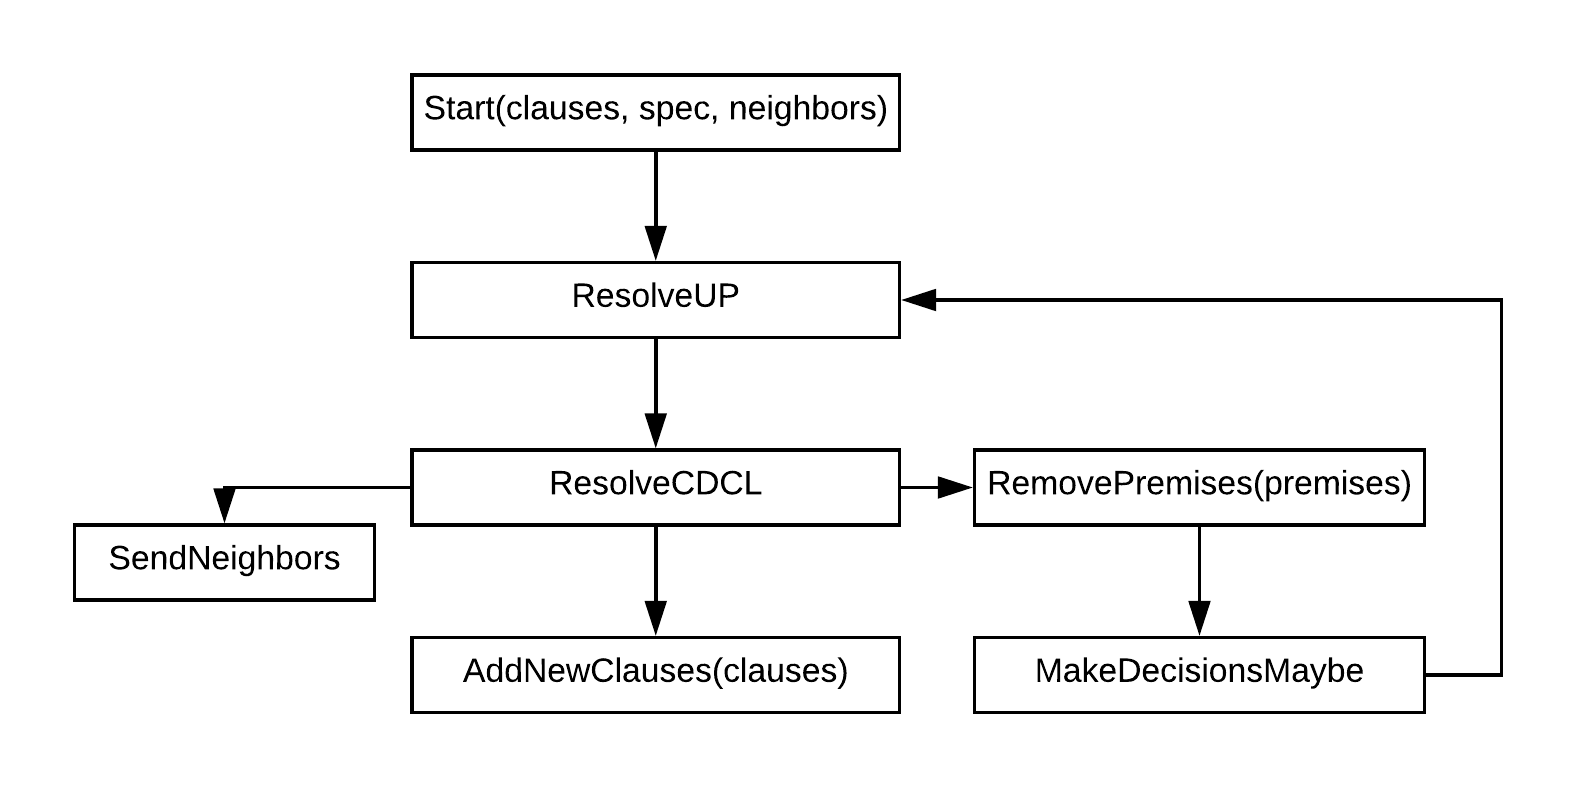
\includegraphics[scale=0.9]{actorProcess.png}
\caption{Сообщения внутри одного актора.}\label{fig:actorProcess}
\end{figure}

На рисунке \ref{fig:actorProcess} описано то, как ведёт себя один актор, для случая статической специализации.
Изначально мы посылаем каждому актору все сообщения с помощью тега \emph{Start}.
\begin{lstlisting}[language=scala]
    case Start(initialClauses, actors) =>
      onReceiveStart(initialClauses, actors)
      self ! ResolveUnitPropagation
\end{lstlisting}

Далее выполняется поиск резолюций -- для этого перебирается клоз, выбирается один литерал, для остальных же ищем соответствующую пару в структуре данных, поддерживающей поиск унифицирующих литералов. Далее применяем унификатор к выбранному литералу, и добавляем его в базу данных внутри этого актора.

После стадии резолюций, начинается выявление конфликтов. Для поиска конфликтов мы должны перебрать пару литералов разного знака, где хотя бы один был выведен на последней итерации, и попытаться подобрать унификатор. Если это получилось, то мы нашли локальный конфликт. В локальном конфликте мы должны проверить существование предположений. Если они есть, то применить правило \emph{CDCL}. Если же их нет, то мы должны взять остаточный клоз и разослать его всем соседям в нашей топологии. Если остаточный клоз тоже пустой, то мы нашли конфликт и необходимо завершить работу всех акторов.

Если на последней итерации стадий \emph{CDCL} и \emph{Unit-Propagation Resolution} не было выявлено новых литералов, то нам нужно сделать предположение. Выбор предположений -- отдельная очень обширная для изучения тема, в которой можно использовать методы обучения с подкреплением, различные простые эвристики. Однако, в рамках данной реализации предположение выбирается случайным образом.

\subsection{Проблема реализации и её решение}
\label{sec:impl-fail}
\begin{figure}
  \begin{prooftree}
      \def\defaultHypSeparation{\hskip .1in}

                      \AxiomC{$[A]^1_1$}
                      \AxiomC{$\neg A \vee D$}
                    \RightLabel{$\confl{1}{}$}
                  \BinaryInfC{$D^1$}
                \RightLabel{$\kshare{1}{2}$}
              \UnaryInfC{$D^2$}

                        \AxiomC{$[A]^1_1$}
                        \AxiomC{$\neg A \vee C$}
                      \RightLabel{$\confl{1}{}$}
                    \BinaryInfC{$C^1$}
                  \RightLabel{$\kshare{1}{2}$}
                \UnaryInfC{$C^2$}
                \AxiomC{$\neg C \vee \neg D$}
                \RightLabel{$\upr{2}{}$}
              \BinaryInfC{$(\neg D)^2$}

              \RightLabel{$\confl{2}{}$}
             \BinaryInfC{$\bot$}
             \RightLabel{$\cdcl{2}{1}$}
             \UnaryInfC{$(\neg A)^2$}
  \end{prooftree}
  \caption{Пример на \emph{CDCL} (вывод $\neg A$)}
  \label{fig:example-cdcl-1}
\end{figure}



\begin{figure} 
  \begin{prooftree}
    \def\defaultHypSeparation{\hskip .0mm}
        \AxiomC{$\alpha (= B^1)$}
        \AxiomC{$\neg B \vee D$}
        \RightLabel{$\confl{1}$}
      \BinaryInfC{$D^1$}
      \RightLabel{$\kshare{1}{2}$}
    \UnaryInfC{$D^2$}
    
             \AxiomC{$\infer[]{(\neg A)^2}{
               \text{(вывод из рис. \ref{fig:example-cdcl-1})}}$
             }
             \RightLabel{$\kshare{2}{1}$}
            \UnaryInfC{$(\neg A)^1$}
            \AxiomC{$(A \vee B)^1$}
            \RightLabel{$\upr{1}{}$}
          \BinaryInfC{$(\alpha = )B^1$}

          \AxiomC{$\neg B \vee C$}
          \RightLabel{$\confl{1}{}$}
        \BinaryInfC{$C^1$}
        \RightLabel{$\kshare{1}{2}$}
        \UnaryInfC{$C^2$}

	    \AxiomC{$\neg C \vee \neg D$}
      \BinaryInfC{$\neg D$}
    
	\BinaryInfC{$\bot$}
  \end{prooftree}
  \caption{Пример на \emph{CDCL} (вторая часть)}
  \label{fig:example-cdcl-2}
\end{figure}

\begin{example}
\label{exmpl:cdcl-fail}
Рассмотрим пример, показанный на рисунках \ref{fig:example-cdcl-1} и \ref{fig:example-cdcl-2}. Здесь находится противоречие для следующего набора формул: \begin{gather*}
			\{ A \vee B
             , \neg A \vee C
             , \neg A \vee D
             , \neg B \vee C
             , \neg B \vee D
             , \neg C \vee \neg D
            \}
		\end{gather*}
 Доказательство ищется в системе из двух акторов, со следующей специализацией $\Psi_1 = \{A, B\}$, $\Psi_2 = \{C, D\}$. Так как все клозы состоят по крайней мере из двух литералов, то нам придётся хотя бы раз воспользоваться правилом \emph{Conflict-Driven Clause Learning}. Проблема этого примера заключается в том, что предположение из одного актора даст нам конфликт в другом акторе, т.е. если мы будем делать \emph{CDCL} только внутри акторов, то наше исчисление не будет полным.
\end{example}

Заметим, что в такой реализации предположения не пересылаются между акторами, и правило \emph{CDCL} может выводить только клозы, состоящие из специализации актора. К сожалению, данной реализации недостаточно, чтобы сохранить полноту. Не составит труда понять, что для набора клозов из примера \ref{exmpl:cdcl-fail} не существует модели, опровергающей этот набор. 

Для решения этой проблемы будем использовать подход, похожий на архитектуру Нельсона-Оппена \cite{Nelson:1979:SCD:357073.357079} для задач о выполнимости формул в теориях (\emph{SMT}-решатели): актор $a$ может послать актору $b$ конъюнкцию литералов, и если $b$ нашёл конфликт, то сообщает об этом $a$, после чего $a$ делает соответствующие откаты.

Для реализации такого подхода будем хранить в каждой вершине дополнительную информацию: список предположений, которые используются вместе с номерами акторов, которые сделали эти предположения. Тогда после использования правила $CDCL$ и получения формулы $\ell_1 \vee \ldots \vee \ell_k$, состоящей из предположений, сделанных в других акторах, мы отправляем каждому из них этот клоз.


\section{Топология}
\begin{figure}[!h]
\centering
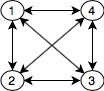
\includegraphics[scale=0.9]{Complete.png}
\caption{Каждый актор шлёт сообщения каждому.}\label{fig:complete}
\end{figure}

\begin{figure}[!h]
\centering
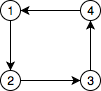
\includegraphics[scale=0.9]{Ring.png}
\caption{Актор посылает сообщение соседу слева}\label{fig:ring}
\end{figure}

Система акторов формирует топологию. Были протестированы два вида реализации: кольцо(рис. \ref{fig:ring}) и полный граф(рис. \ref{fig:complete}). Алгоритм с топологией в виде кольца назовём \emph{EAR}, а с топологией полного графа --- \emph{EAC}. 

На первый взгляд может показаться, что топология полного графа будет иметь плохую производительность, однако стоит заметить, что каждый отдельный актор решает трудную комбинаторную задачу, а количество сообщений от одного актора другому не так велико на практике, чтобы иметь значительный вес в оценке производительности.

\section{Доказательство полноты по опровержению для реализации}
Для того, чтобы понять, что реализация работает, необходимо показать, что если существует вывод некоторой формулы в исчислении \emph{Expertised Conflict Resolution}, то какое-то доказательство найдётся и нашим алгоритмом. 

\begin{theorem}
Пусть существует некоторый вывод формулы $\phi^i$ в исчислении \emph{ECR}. Тогда алгоритм \emph{EAC} построит это доказательство за конечное время.
\end{theorem}
\begin{proof}
Будем доказывать по структуре графа доказательства в \emph{ECR}.
\begin{enumerate}[label=$\star$]
	\item \emph{База.} Вершина без входящих в неё рёбер. В такой вершине записан начальный клоз в виде $\xi^i$. Это означает, что актор $i$ специализируется на литерале $\xi$. И мы отправим ему сообщение $Start$, в котором будет содержаться выражение $\xi$.
    \item \emph{Переход.} Вершина получена одним из четырёх правил вывода: 
    \begin{enumerate}
      \item \emph{Unit-Propagation Resolution.} Если в \emph{ECR} вывод $\xi^i$ заканчивается применением правила \emph{Unit-Propagation Resolution} в акторе $i$, то этот актор найдёт применение правила, посколько он перебирает все возможные варианты. 
      \item \emph{Conflict.} Посколько на стадии \emph{ResolveConflicts} актор находит все возможные варианты конфликтов, а по предположению индукции все предпосылки уже выведены, то данное применение правила тоже будет найдено.
      \item \emph{Conflict-Driven Clause Learning.} Поскольку в нашей реализации предположения могут пересылаться с помощью правила \emph{Knowledge Sharing} и в следующем пункте мы покажем, что это правило сохраняет полноту по опровержению в рамках нашего алгоритма, то каждый актор находит все возможные выводы правила \emph{CDCL} на стадии \emph{ResolveCDCL} и сообщает о выведенных клозах другим акторам.
      \item \emph{Knowledge Sharing.} В исчислении \emph{Expertised Conflict Resolution} правило \emph{Knowledge Sharing} может применяться в произвольных местах, однако в нашей реализации это происходит только когда актор смог сократить часть клоза, на которой он специализируется. Для обоснования полноты по опровержению заметим, что применение правила \emph{Knowledge Sharing} имеет смысл только непосредственно после применения правил \emph{Conflict} и \emph{Conflict-Driven Clause Learning}. Это можно показать более формально индукцией по структуре доказательства.
    \end{enumerate}
\end{enumerate}
\end{proof}

% \section{Оценка сложности для задачи \emph{Принцип Дирихле}}
% В резолюционном исчислении сложно оценивать сложность общего алгоритма, поэтому чаще всего оценивается на конкретных задачах. Одной из таких классических задач является \emph{Принцип Дирихле}. 
% \texttt{TODO: написать здесь доказательство оценки}
\section{Экспериментальные результаты}

Реализации тестировались на задачах из архива \emph{TPTP}. Множество тестов содержит $1606$ задач без равенства из класса Бернайса-Шейфенкеля. 

Запуски производились на кластере из $200$ машин, предоставленном университетом Майями \cite{StarExec}. На машинах были процессоры \emph{Intel Xeon E5-2609} частотой $2.4$ ГГц, и $128$ Гб ОЗУ.

Было установлено ограничение в $300$ секунд реального времени. Сравнивались $3$ версии алгоритма:
\begin{itemize}[label=*]
	\item \emph{EAC1} -- версия с одним актором. Эта реализация эквивалентна алгоритму \emph{EPCR} \cite{DBLP:journals/corr/ItegulovSP17}. Данная версия решила $880$ задач и считается базовой.
    \item \emph{EAC2} -- версия с двумя акторами дала прирост в $39$ задач по сравнению с базовой, и решила $919$ задач.
    \item \emph{EAC4} -- версия с четырьмя акторами и топологией полного графа. Данная версия дала прирост $66$ задача по сравнению с базовой, решив $956$ задач из $1606$.
\end{itemize}


\begin{figure}[!h]
\centering
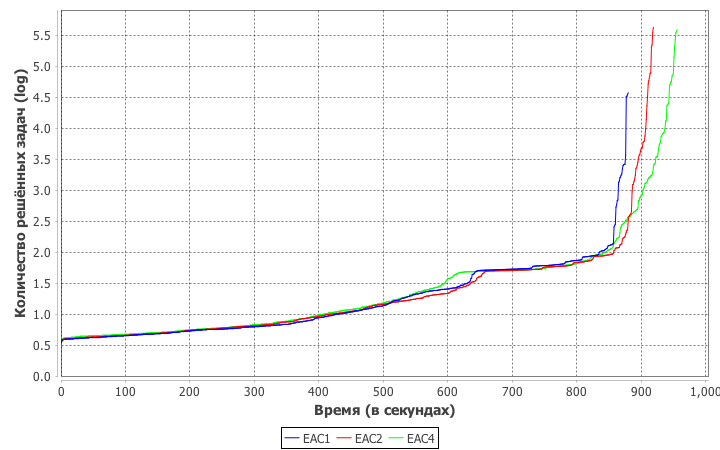
\includegraphics[scale=0.6]{chart.png}
\caption{Сравнение результатов работы нескольких САДТ.}\label{fig:chart}
\end{figure}

На рисунке \ref{fig:chart} показана производительность трёх реализаций, описанных выше. Для удобства была взята логарифмическая шкала по временной оси. Видно, что для ограничения по времени до $10$ секунд акторные модели не дают значительного роста в производительности. Однако на $300$ секундах увеличение количества рабочих акторов даёт значительный прирост в количестве решённых задач.
% для $1$, $2$, и $4$ акторов. Для удобства по оси \textquote{количества решённых задач} была взята логарифмическая шкала. Версия решения с одним актором соответствует алгоритму \emph{EPCR} , который основан на чистом исчислении \emph{Conflict Resolution}. Версия с одним актроом успела за 300 секунд найти опровергающие модели для 880 задач из 1606 доступных в архиве \emph{TPTP}. Для двух акторов -- 919 задач. Для четырёх -- 946.

\newpage
\section{Выводы к третьей главе}
\begin{enumerate}
	\item Описан алгоритм на основе исчисления из главы \ref{sec:chap2}
    \item Доказана его полнота по опровержению
    \item Показана его производительность в сравнении с алгоритмом \emph{EPCR}.
\end{enumerate}

\end{document}
